\section{Ablation Study}

\subsection{Framework Ablation}

\begin{figure*}[htbp]
    \centering
    \begin{subfigure}[t]{0.4\textwidth}
      \centering
      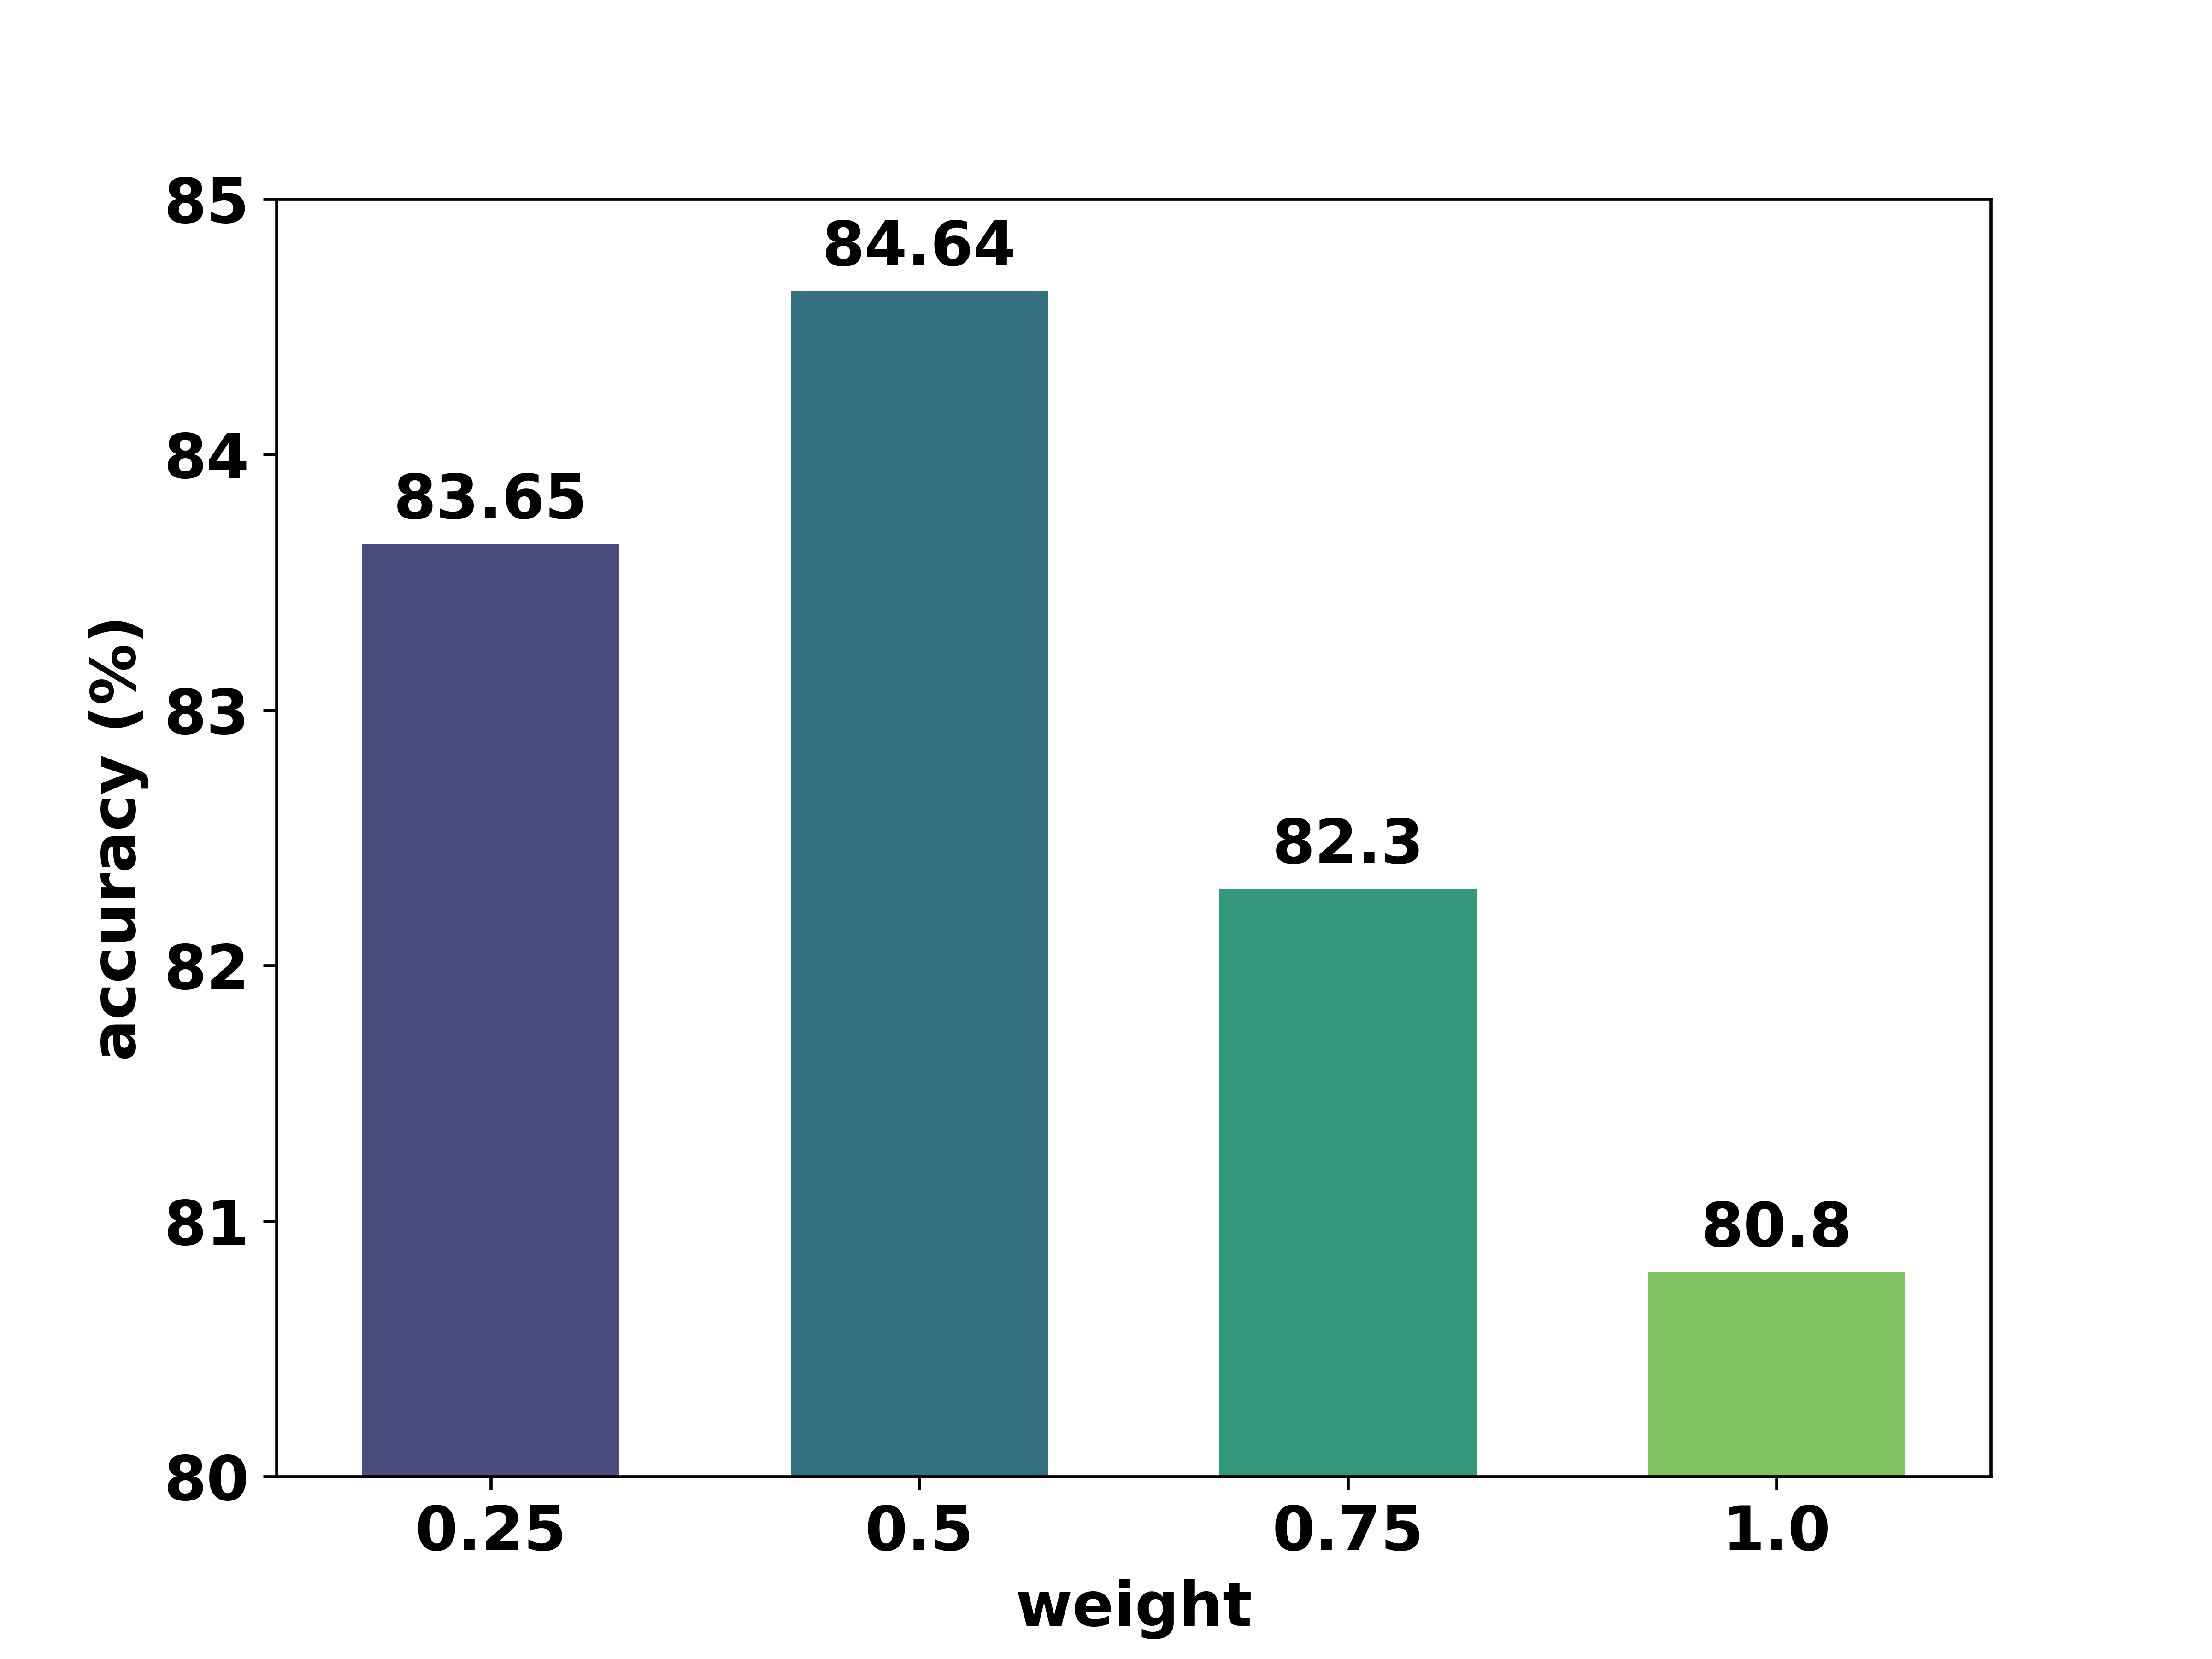
\includegraphics[width=\linewidth]{images/accuracy_vs_weight.png}
      \caption{Effect of the auxiliary loss weight, $\lambda$.}
      \label{fig:weight}
    \end{subfigure}%
  \hspace{0.05\textwidth} % Adjust space here
    \begin{subfigure}[t]{0.4\textwidth}
      \centering
      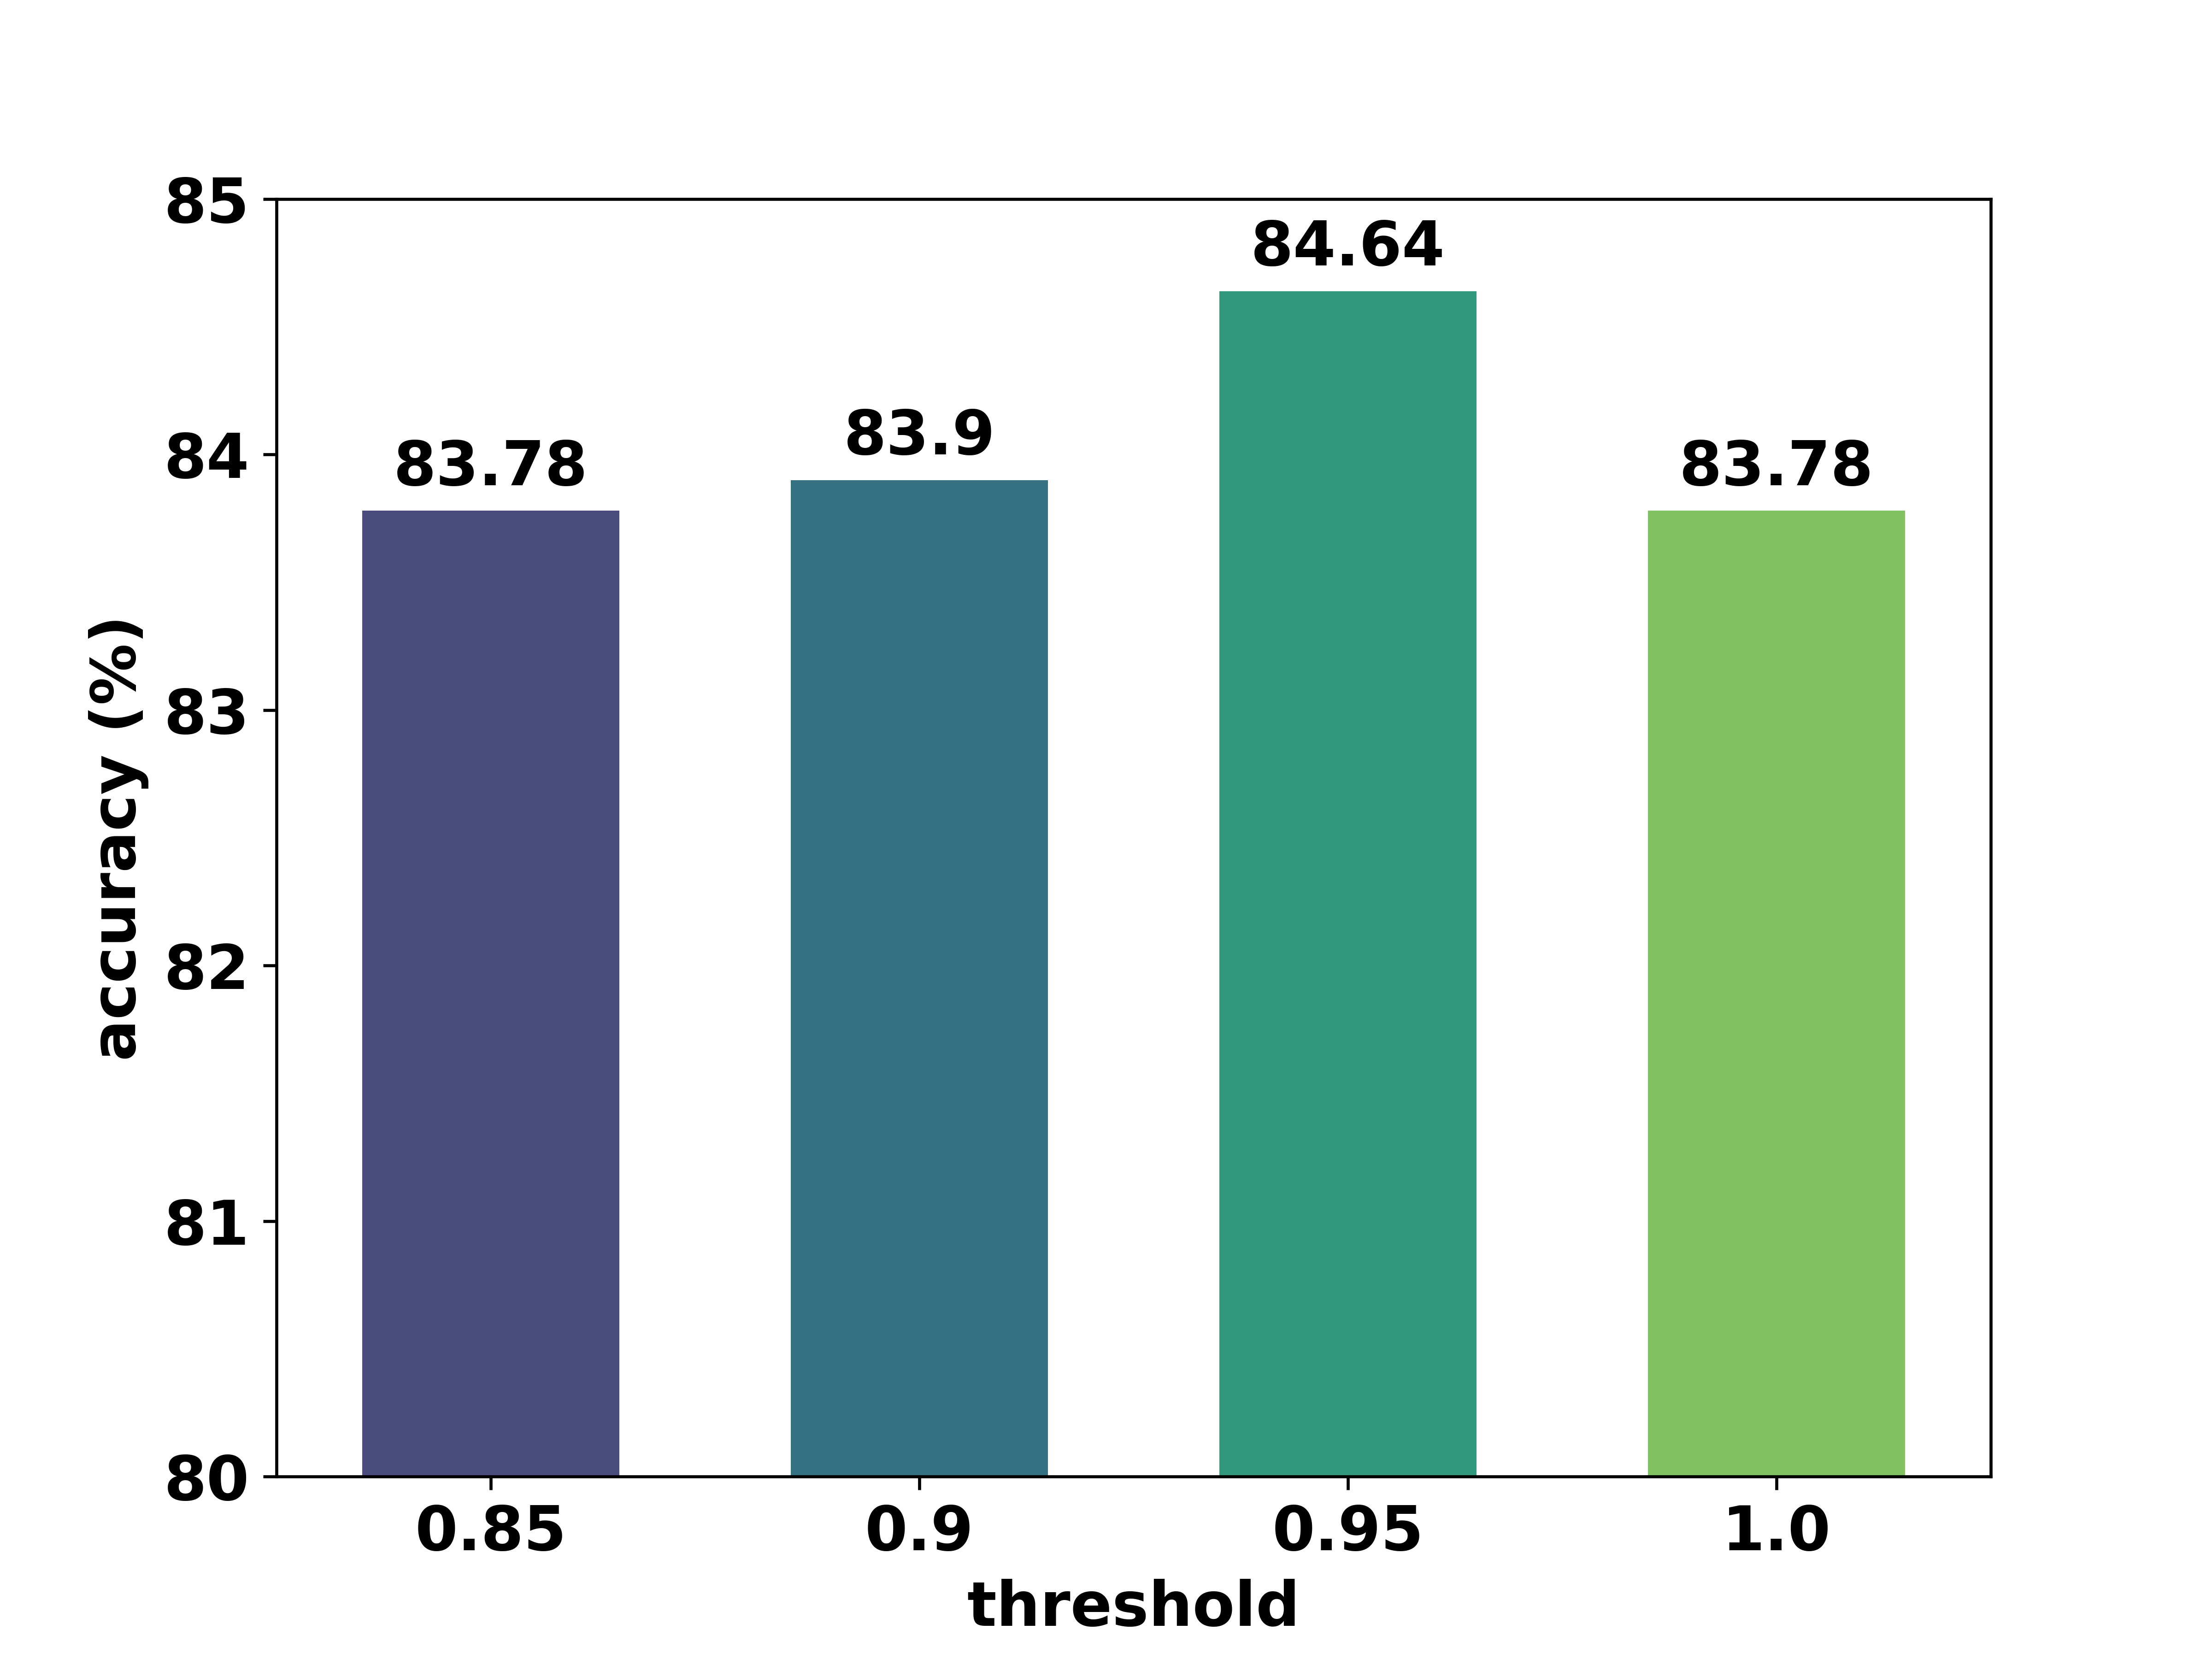
\includegraphics[width=\linewidth]{images/accuracy_vs_threshold.png}
      \caption{Effect of the pseudo labels threshold, $\tau$.}
      \label{fig:threshold}
    \end{subfigure}
    \caption{Effects of different hyperparameters on model performance.}
  \end{figure*}

We conduct extensive ablation studies to evaluate the effectiveness of our method against the PL algorithm with random initialization and RLPL without PLs. Results in Table \ref{table:ablation} demonstrate the consistent superiority of RLPL across diverse datasets and label regimes. The PL with random initialization exhibits limited performance, particularly struggling with low-label scenarios (e.g., 30.49\% and 11.19\% accuracy with 250 labels), highlighting the importance of proper initialization for PL's reliability. 

RLPL without pseudo labeling shows substantial improvements over the baseline, achieving notable gains on STL-10 (83.20\% vs 53.34\%) and SVHN (71.25\% vs 11.19\% for 250 labels), validating the effectiveness of our representation learning strategy. The full RLPL framework, integrating both representation learning and pseudo labeling, consistently achieves the highest performance across all configurations, with particularly strong improvements in low-label settings (e.g., 48.93\% on CIFAR-10 with 250 labels, an 18.44\% improvement). This comprehensive performance advantage is reflected in the average accuracy across all settings, demonstrating RLPL's robust capability, especially in label-scarce scenarios where traditional approaches typically falter.

\subsection{Ablation on Noisy Teacher}

\begin{table}[!htbp]
\centering
\begin{tabular}{cc}
\hline
\textbf{Method} & \textbf{Accuracy (\%)} \\
\hline
Noisy Student    & 84.54 $\pm$ 0.05 \\
Noiseless Teacher & 84.59 $\pm$ 0.02 \\
Noisy Teacher     & 84.63 $\pm$ 0.02 \\
\hline
\end{tabular}
\caption{Input types ablation for pseudo labeling.}
\label{table:noise}
\end{table}

We investigate the impact of noisy samples (weakly augmented) in both teacher and student networks. Table \ref{table:noise} presents the average performance of five different runs for three configurations: the noisy student, the noiseless teacher, and our proposed noisy teacher method. While the differences are subtle, they reveal interesting patterns in model behavior. The noisy student achieves 84.54\% accuracy with a standard deviation of 0.05, suggesting some variability in performance. When we remove noisy samples from the teacher network, we observe a marginal improvement to 84.59\% with reduced variance. Our proposed approach achieves the highest accuracy at 84.63\% with consistently low variance. These results suggest that weak augmentation in the teacher network inputs can provide additional regularization benefits.


% \subsection{Projector Dimensionality}

\section{Parameter Studies}

\subsection{Weight of the Auxiliary Loss}

We modify the weight of auxiliary loss, $\lambda$, from $0.25$ to $1.0$ with an increment of $0.25$. We observe that there is a strong effect of the weight on model performance. For weights other than $0.50$, the test accuracy declines as we move further from this value. The outputs are shown in Figure \ref{fig:weight}.

\subsection{Threshold for Pseudo Labels}

We vary the threshold, $\tau$, from $0.85$ to $1.0$ with an increment of $0.05$. We observe that the highest accuracy is obtained at $0.95$, and it keeps decreasing for a lower threshold value. Again, the accuracy decreases for a threshold value of $1.0$. For any threshold other than $0.95$, the accuracy drops below 84.0\%. The outputs are shown in Figure \ref{fig:threshold}.
